%%%%%%%%%%%%%%%%%%%%%%%%%%%%%%%%%%%%%%%%%%%%%%%%%%%%%%%%%%%%%%%%%%%%%%%%%%%%%%%%%%%%%%%%
%%%%%%%%%%%%%%%%%%%%%%%%   Template de rapport CUINET Antoine   %%%%%%%%%%%%%%%%%%%%%%%%
%%%%%%%%%%%%%%%%%%%%%%%%%%%%%%%%%%%%%%%%%%%%%%%%%%%%%%%%%%%%%%%%%%%%%%%%%%%%%%%%%%%%%%%%

\documentclass[11pt,a4paper, french]{report} % Type du document (ici un rapport)

%%% Paquets utiles
\usepackage[T1]{fontenc} % caractères français
\usepackage[utf8]{inputenc} % accents
\usepackage[french,english]{babel} % langues
\usepackage{xcolor} % couleurs
\usepackage{blindtext}
\usepackage{fancyhdr} % pour la pagination
\usepackage{lastpage} % pour avoir le nombre de pages totales du document
\usepackage{fourier}
\usepackage{multicol} % pour avoir multiples colonnes localement
\usepackage{amsmath,amssymb,amsthm,delarray,indentfirst,numprint,manfnt}
\usepackage{soulutf8}
\usepackage{eurosym}
\usepackage{datatool}
\usepackage{fontawesome5}%pour les icons
\usepackage{nopageno} % pagination
\usepackage{soul, lettrine}
\usepackage{ipa,indentfirst,epic,ecltree}
\usepackage{graphicx} % mettre des images
\usepackage{floatrow} % pour les images (redéfinitions)
\usepackage{caption} % pour les images
\usepackage{wrapfig} % images dans un text
\usepackage[most]{tcolorbox}
\usepackage[rightcaption]{sidecap} % mettre des images à gauche et à droite d'un texte
\usepackage{geometry} % pour les marges
\usepackage{wrapfig}
\usepackage{moreverb} % verbatim en box ebvironnement boxedverbatim
\usepackage{verbatim} % texte préformaté
\usepackage{fancyvrb} % verbatim mais en mieux on l'utilise avec \begin{BVerbatim}, et cette fois on peut centrer
\usepackage{authblk}
\usepackage{wasysym}
\usepackage{listings}
\usepackage{titlesec} % pour enlever le mot "chapitre"
\usepackage{lipsum} % ajouter du texte dans les dessins tikz
\usepackage{tikz} % pour dessiner
\usepackage{pgf}
\usepackage[linesnumbered,algosection]{algorithm2e} %Pour le PDL
\usepackage{mdframed}
\usepackage{enumitem}
\usepackage{lmodern,eso-pic,fullpage}  
\usepackage{stackengine,scalerel}
\usepackage[colorlinks=true, % colorise les liens
            urlcolor=black, % couleur des hyperliens
            linkcolor=black, % couleur des liens internes aux documents (index, figures, tableaux, equations,...)
            breaklinks=true, % permet les retours à la ligne pour les liens trop longs
            citecolor= black, % couleur des liens vers les references bibliographiques
            plainpages=false  %pour palier à "Bookmark problems can occur when you have duplicate page numbers, for example, if you have a page i and a page 1."
            ]{hyperref} % pour utiliser des liens internes, càd en réferencant une partie en peut mettre un lien vers celle-ci et ça avec \hyperref[nom du label]{le texte où y'aura le lien} sans oublier de mettre le \label{nom du label} sur la partie que vous voulez réferencer
\usepackage[bottom]{footmisc} % remettre le compteur de footnote à 0 par section
\counterwithin*{footnote}{section} %numerote les footnote par section

%%% set-up francais (espaces et notes en bas de page)
\frenchbsetup{AutoSpaceFootnotes,FrenchFootnotes}%

%%% indentations
\newlength{\savedparindent}
\setlength{\savedparindent}{\parindent}
\newcommand{\restoreparindent}{\setlength{\parindent}{\savedparindent}}

%%% permet de changer le nom de la liste des figures et celui des tableaux
\addto\captionsfrench{%
  \renewcommand{\listfigurename}{~~~LISTE DES FIGURES}%
  \renewcommand{\listtablename}{~~~LISTE DES TABLEAUX}%
  \renewcommand{\listalgorithmcfname}{~~~LISTE DES ALGORITHMES}%
  \renewcommand{\bibname}{~~~V -~BIBLIOGRAPHIE}% change le nom de la bibliographie
}

\counterwithin*{footnote}{section} % numerote les footnote par section
\setcounter{secnumdepth}{3} % affiche le sommaire jusqu'à une profondeur de 3

\titleformat{\chapter}[display]{\normalfont\bfseries}{}{0pt}{\Huge} % format du titre
% \addto{\captionsfrench}{
%     \renewcommand*{\chapternamename}{Partie}}

%%% pour le glossaire
\newcommand{\sortitem}[2][]{%
  \DTLnewrow{list}%
  \DTLnewdbentry{list}{description}{\textbf{#1~:\xspace}\xspace#2}%**
  }

\newenvironment{sortedlist}{%
  \DTLifdbexists{list}{\DTLcleardb{list}}{\DTLnewdb{list}}%
  }%
  {%
  \DTLsort{description}{list}% Sort list
  \begin{description}[labelindent=-0.5em]%
    \DTLforeach*{list}{\theDesc=description}{%
    \item\theDesc}% Print each item
  \end{description}}

%%% tout cela sert pour la position des logos des entreprises
\newcommand{\blap}[1]{\vbox to 0pt{#1\vss}}
\newcommand\AtUpperLeftCorner[3]{\put(\LenToUnit{#1},\LenToUnit{\dimexpr\paperheight-#2}){\blap{#3}}}
\newcommand\AtTopCenterPage[2]{\put(\LenToUnit{.5\paperwidth},\LenToUnit{\dimexpr\paperheight-#1}){\blap{\hbox to 0pt{\hss#2\hss}}}}
\newcommand\AtUpperRightCorner[3]{\put(\LenToUnit{\dimexpr\paperwidth-#1},\LenToUnit{\dimexpr\paperheight-#2}){\blap{\llap{#3}}}}
\lstset{basicstyle=\ttfamily, mathescape=true} % utiliser le module maths

%%% permet d'afficher les numéros des titres selon un certain style
\renewcommand\thechapter{\Roman{chapter}} % ici chiffres romains pour les chapitres (se voit que dans le sommaire)
\renewcommand\thesection{\Alph{section}} % ici lettres majuscules pour les sections
\renewcommand\thesubsection{\thesection\,-\,\arabic{subsection}} % ici chiffres arabes pour les sous-sections (\thesection-  pour mettre la section est un tiret entre)

% Pour les pénalités :
\interfootnotelinepenalty=150 % note de bas de page
\widowpenalty=150 % veuves et orphelines
\clubpenalty=150

%%% bas/haut de page
\fancypagestyle{plain}{ % redéfinition de ce style pour l'affichage de la pagination sur les pages ou sont défini les chapitres
  \renewcommand{\headrulewidth}{0pt} % ligne horizontale du haut de page
  \renewcommand{\footrulewidth}{0.5pt} % ligne horizontale en bas de page 
}  
\pagestyle{fancy}
\fancyhead[L]{}

\renewcommand{\headrulewidth}{0pt} % ligne horizontale du haut de page
\renewcommand{\footrulewidth}{0.5pt} % ligne horizontale en bas de page
\pagenumbering{arabic} % pour la numérotation des pages en chiffres
\setlength{\headheight}{25.33461pt}

%%% Définition des couleurs: \textcolor{camouflagegreen}{\textsc{...}} pour l'utiliser
\definecolor{babyblueeyes}{rgb}{0.63, 0.79, 0.95} %joli bleu
\definecolor{blush}{rgb}{0.87, 0.36, 0.51} %joli rose
\definecolor{chromeyellow}{rgb}{1.0, 0.65, 0.0} %joli jaune\orange pour julie 
\definecolor{camouflagegreen}{rgb}{0.47, 0.53, 0.42} %joli vert
\definecolor{cardinal}{rgb}{0.77, 0.12, 0.23} %joli rouge
\definecolor{purple}{rgb}{0.57, 0.36, 0.51} %joli violet
\definecolor{auburn}{rgb}{1.57, 0.62, 0.12} % marron

%%% Définition de commandes utiles
\newtcbox{\mybox}{colback=red!5!white, colframe=red!75!black} % encadré rouge
\newcommand{\HRule}{\rule{\linewidth}{0.5mm}} % utiliser "\HRule" pour faire une ligne noir
\newcommand{\frule}[1][\textwidth]{\rule{#1}{0.4mm}} % utiliser \frule[taille] pour faire ligne noir
\newcommand{\maj}[1]{\uppercase{#1}}% permet de mettre en majuscule
\newcommand{\hlc}[2][yellow]{{\sethlcolor{#1} \hl{#2}}} % pour surligner en jaune: \hlc  pour l'utiliser
\newcommand{\g}[1]{\og#1 \fg} % guillemets, s'utilise: \g{} 



%%%%%%%%%%%%%%%%%%%%%%%%%%%%%%%%%%%%%%%%%%%%%%%%%%%%%%%%%%%%%%%%%%%%%%%%%%%%%%%%%%%%%%%%
%%%%%%%%%%%%%%%%%%%%%%%%%%%%%%%   Modifications here   %%%%%%%%%%%%%%%%%%%%%%%%%%%%%%%%%
%%%%%%%%%%%%%%%%%%%%%%%%%%%%%%%%%%%%%%%%%%%%%%%%%%%%%%%%%%%%%%%%%%%%%%%%%%%%%%%%%%%%%%%%

%%% Définitions des commandes personnalisées 
\newcommand{\nom}[1]{\textsc{Les Tours Infernales }}% pour le nom de l'agence 
\newcommand{\adr}[1]{\href{https://goo.gl/maps/6j9bxdbWx3H1bwSYA}{Rue du Bois de la Courbe – ZAC Valentin Nord – 25870 CHATILLON LE DUC}}% pour l'adresse de l'agence \adr\~ pour l'utiliser
\newcommand{\wpress}[1]{\textsc{WordPress}}% nom de vertical
\newcommand{\ginko}[1]{\href{https://www.ginko.voyage/}{\textsc{Ginko}}}% site ginko

\title{ \LARGE{Rapport de projet de Programmation Objet Avancée}\\[0,5cm] % Titre
        \Huge{Les Tours Infernales}}

\author{ \\ \huge{\textbf{Antoine CUINET}} \\ 
        ~\\
        \textbf{Tristan AMIOTTE-SUCHET}} % Auteur
\newcommand{\anneeUniversitaire}{Année 2023–2024} % Date

\fancyhead[R]{\textbf{\mbox{LES TOURS INFERNALES}}\\
~} % met le haut de page à vide

\fancyfoot[L]{POA Informatique~-~L2}
\fancyfoot[R]{\leftmark} % affiche en pied de page le nom du chapitre
\renewcommand{\chaptermark}[1]{\markboth{#1}{}} % enlève le mot "chapitre X" dans le pied de page avant le nom du chapitre
\fancyfoot[C]{\textbf{page \thepage~sur~\pageref{LastPage}}} % numérote les pages



%%%%%%%%%%%%%%%%%%%%%%%%%%%%%%%%%%%%%%%%%%%%%%%%%%%%%%%%%%%%%%%%%%%%%%%%%%%%%%%%%%%%%%%%
%%%%%%%%%%%%%%%%%%%%%%%%%%%%   Le PDL (pseudo-language)   %%%%%%%%%%%%%%%%%%%%%%%%%%%%%%
%%%%%%%%%%%%%%%%%%%%%%%%%%%%%%%%%%%%%%%%%%%%%%%%%%%%%%%%%%%%%%%%%%%%%%%%%%%%%%%%%%%%%%%%

%pour les entiers
\SetKwProg{FnInt}{ \textcolor{blush}{entier} \textcolor{babyblueeyes}{fonction}}{}{\textcolor{babyblueeyes}{fin Fonction}}

%pour les caractères
\SetKwProg{FnChar}{ \textcolor{blush}{car} \textcolor{babyblueeyes}{fonction}}{}{\textcolor{babyblueeyes}{fin Fonction}}

%pour les booléens
\SetKwProg{FnBool}{ \textcolor{blush}{booléen} \textcolor{babyblueeyes}{fonction}}{}{\textcolor{babyblueeyes}{fin Fonction}}

%pour les tableaux de dimension 1
\SetKwProg{FnTab}{\textcolor{blush}{tab[]} \textcolor{babyblueeyes}{fonction}}{}{\textcolor{babyblueeyes}{fin Fonction}}

%pour les tableaux de caractères
\SetKwProg{FnCharTab}{\textcolor{blush}{car[ ]} \textcolor{babyblueeyes}{fonction}}{}{\textcolor{babyblueeyes}{fin Fonction}}

%pour les positions
\SetKwProg{FnPos}{ \textcolor{blush}{Position} \textcolor{babyblueeyes}{fonction}}{}{\textcolor{babyblueeyes}{fin Fonction}}

%pour les matrices de dimension 2
\SetKwProg{FnMat}{\textcolor{blush}{tab[][]} \textcolor{babyblueeyes}{fonction}}{}{\textcolor{babyblueeyes}{fin Fonction}}

%pour les réels
\SetKwProg{FnReel}{\textcolor{blush}{réel} \textcolor{babyblueeyes}{fonction} }{}{\textcolor{babyblueeyes}{fin Fonction}}

%Actions
\SetKwProg{Act}{\textcolor{chromeyellow}{action}}{}{\textcolor{chromeyellow}{fin Action}}

%html
\SetKwProg{html}{<\textcolor{blue}{html}>}{}{</\textcolor{blue}{html}>}

%head
\SetKwProg{head}{<\textcolor{blue}{head}>}{}{</\textcolor{blue}{head}>}

%body html
\SetKwProg{body}{<\textcolor{blue}{body}>}{}{</\textcolor{blue}{body}>}

%body css
\SetKwProg{bodycss}{\textcolor{blue}{body} \textcolor{blue}{\textcolor{auburn}{ $\{$ }}}{}{\textcolor{auburn}{$\}$}}

%div container
\SetKwProg{div}{<\textcolor{blue}{div} \textcolor{cyan}{class}=\textcolor{auburn}{“container”}>}{}{</\textcolor{blue}{div}>}

% . CSS
\SetKwProg{point}{\textcolor{auburn}{.}}{}{\textcolor{auburn}{ $\} $ }}

% @keyframes CSS
\SetKwProg{keyf}{\textcolor{purple}{@keyframes}}{}{\textcolor{auburn}{ $\} $ }}

%algo
\RestyleAlgo{boxed}
\SetAlgoSkip{1cm}

\SetKwProg{tab}{\textcolor{blue}{\{}}{}{\textcolor{blue}{\}}}


%%% Début du document ici
\begin{document}%
\selectlanguage{french}
\hypersetup{pdfborder=0 0 0}% permet de ne pas avoir un encadré rouge autour des liens

%%%%%%%%%%%%%%%%%%%%%%%%%%%%%%%%%%%%%%%%%%%%%%%%%%%%%%%%%%%%%%%%%%%%%%%%%%%%%%%%%%%%%%%%%%%%%%%%%
%%%%%%%%%%%%%%%%%%%%%%%%%%%%%%%%%%%%%%%%   COUVERTURE  %%%%%%%%%%%%%%%%%%%%%%%%%%%%%%%%%%%%%%%%%%
%%%%%%%%%%%%%%%%%%%%%%%%%%%%%%%%%%%%%%%%%%%%%%%%%%%%%%%%%%%%%%%%%%%%%%%%%%%%%%%%%%%%%%%%%%%%%%%%%
\makeatletter % permet d'afficher le titre (sinon on n'affiche pas le texte)
\begin{titlepage} % génération de la première de couverture
  \enlargethispage{3cm} % permet de pouvoir écrire plus bas dans la page 

  \AddToShipoutPicture{ 
  \AtUpperLeftCorner{2cm}{3.5cm}{
\includegraphics[width=6.5cm]{assets/pictures/logos/logo_ufr.png}} % Logo à gauche en haut
  \AtUpperRightCorner{2cm}{3.5cm}{
\includegraphics[width=8.5cm]{assets/pictures/logos/logo_ubfc.png}}
  \AtUpperRightCorner{3cm}{6.5cm}{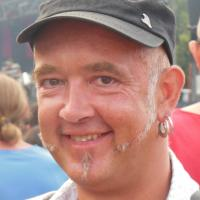
\includegraphics[width=2cm]{assets/pictures/logos/PAM.jpeg}}
  % \AtUpperRightCorner{2cm}{2cm}{\includegraphics[width=7cm]{assets/pictures/logos/logo_koredge.png}}
  }

  \begin{center}	
    \vspace*{7.5cm}
    \textsc{\@title} \\
    \vspace*{0,5cm} 
    \HRule%
    \vspace*{0,5cm}
    \large{\@author} \\ 
    \vspace*{0.6cm}
    \anneeUniversitaire\\
    \vspace*{1cm}
    % \includegraphics[width=12cm]{assets/pictures/photo_Koredge.jpg}
  \end{center}

  \vspace*{3cm}
  \noindent
  \large{\textbf{Groupe de TP:} TP2A~- CMI}\\
  \large{\textbf{Année de licence:} Licence 2~- Informatique}\\
  \large{\textbf{Unité d’enseignement:} Programmation Objet Avancée}\\
  \vspace*{0cm}

  % \noindent
  % \large{\textbf{Superviseur académique:} \textsc{DADEAU} Frédéric}
  
  % \vspace*{1cm}
  % \noindent
  % \large{\textbf{Établissement de formation:} Première année de Licence en CMI Informatique  au sein de l'Université de Franche-Comté (Année 2022-2023)} \\
  % \vspace*{0cm}

  % \noindent
  % \large{\textbf{Agence d’accueil:} Agence \nom\ }\\
  % \adr%
    
\end{titlepage}
\ClearShipoutPicture% empèche les logos de se répétés sur les autres pages
\newpage

%%%%%%%%%%%%%%%%%%%%%%%%%%%%%%%%%%%%%%%%%%%%%%%%%%%%%%%%%%%%%%%%%%%%%%%%%%%%%%%%%%%%%%%%%%%%%%%%%
%%%%%%%%%%%%%%%%%%%%%%%%%%%%%%%%%%%%%%%   PAGE DE GARDE  %%%%%%%%%%%%%%%%%%%%%%%%%%%%%%%%%%%%%%%%
%%%%%%%%%%%%%%%%%%%%%%%%%%%%%%%%%%%%%%%%%%%%%%%%%%%%%%%%%%%%%%%%%%%%%%%%%%%%%%%%%%%%%%%%%%%%%%%%%

\thispagestyle{empty} % ne pas numéroter la page
\setcounter{page}{0} % commencer la numérotation juste après
\null% permet de faire une page vide
\newpage

%%%%%%%%%%%%%%%%%%%%%%%%%%%%%%%%%%%%%%%%%%%%%%%%%%%%%%%%%%%%%%%%%%%%%%%%%%%%%%%%%%%%%%%%%%%%%%%%%
%%%%%%%%%%%%%%%%%%%%%%%%%%%%%%%%%%%%%%%   PAGE DE TITRE  %%%%%%%%%%%%%%%%%%%%%%%%%%%%%%%%%%%%%%%%
%%%%%%%%%%%%%%%%%%%%%%%%%%%%%%%%%%%%%%%%%%%%%%%%%%%%%%%%%%%%%%%%%%%%%%%%%%%%%%%%%%%%%%%%%%%%%%%%%

% \makeatletter % permet d'afficher le titre (sinon on n'affiche pas le texte)
% \begin{titlepage} % génération de la première de couverture
%   \enlargethispage{3cm}
%   \begin{center}	
%     \vspace*{5cm}
%     \textsc{\@title} \\
%     \vspace*{0,5cm}
%     \HRule%
%     \vspace*{0,5cm}
%     \large{\@author} \\
%     \vspace*{0.2cm}
%     \anneeUniversitaire\\
%     \vspace*{1cm}
%   \end{center}
%   \vspace*{5.5cm}
%   \noindent
%   \large{\textbf{Directeur de stage:} \textsc{LOIZEAU} Julien}\\
%   \vspace*{0cm}

%   \noindent\large{\textbf{Superviseur académique:} \textsc{DADEAU} Frédéric}
%   \vspace*{1.5cm}

%   \noindent
%   \large{\textbf{Établissement de formation:} Première année de Licence en CMI Informatique  au sein de l'Université de Franche-Comté (Année 2022-2023)}\\
%   \vspace*{0cm}

%   \noindent
%   \large{\textbf{Agence d’accueil:} Agence \nom\ }\\
%   \adr%
  
% \end{titlepage}
\newpage

%%%%%%%%%%%%%%%%%%%%%%%%%%%%%%%%%%%%%%%%%%%%%%%%%%%%%%%%%%%%%%%%%%%%%%%%%%%%%%%%%%%%%%%%%%%%%%%%%
%%%%%%%%%%%%%%%%%%%%%%%%%%%%%%%%%%%%%%%   REMERCIEMENTS  %%%%%%%%%%%%%%%%%%%%%%%%%%%%%%%%%%%%%%%%
%%%%%%%%%%%%%%%%%%%%%%%%%%%%%%%%%%%%%%%%%%%%%%%%%%%%%%%%%%%%%%%%%%%%%%%%%%%%%%%%%%%%%%%%%%%%%%%%%
%%% décommenter ici pour rajouter les remeciements
% \input{assets/remerciements}

%%%%%%%%%%%%%%%%%%%%%%%%%%%%%%%%%%%%%%%%%%%%%%%%%%%%%%%%%%%%%%%%%%%%%%%%%%%%%%%%%%%%%%%%%%%%%%%%%
%%%%%%%%%%%%%%%%%%%%%%%%%%%%%%%%%%%%%%%%%   SOMMAIRE  %%%%%%%%%%%%%%%%%%%%%%%%%%%%%%%%%%%%%%%%%%%
%%%%%%%%%%%%%%%%%%%%%%%%%%%%%%%%%%%%%%%%%%%%%%%%%%%%%%%%%%%%%%%%%%%%%%%%%%%%%%%%%%%%%%%%%%%%%%%%%
\cleardoublepage%
\phantomsection% permet de rediriger au bon endroit (sinon redirige vers sommaire)
\large%
\renewcommand{\contentsname}{~~~SOMMAIRE}%
\tableofcontents%
%\addcontentsline{toc}{chapter}{i~~~~~~SOMMAIRE}%
% \normalsize%

%%%%%%%%%%%%%%%%%%%%%%%%%%%%%%%%%%%%%%%%%%%%%%%%%%%%%%%%%%%%%%%%%%%%%%%%%%%%%%%%%%%%%%%%%%%%%%%%%
%%%%%%%%%%%%%%%%%%%%%%%%%%%%%%%%%%%%%   LISTE DES FIGURES  %%%%%%%%%%%%%%%%%%%%%%%%%%%%%%%%%%%%%%
%%%%%%%%%%%%%%%%%%%%%%%%%%%%%%%%%%%%%%%%%%%%%%%%%%%%%%%%%%%%%%%%%%%%%%%%%%%%%%%%%%%%%%%%%%%%%%%%%
\cleardoublepage%
\phantomsection% 
\addcontentsline{toc}{chapter}{i~~~~~~LISTE DES FIGURES}% Pardon pour le i~~~~~~
\listoffigures%

%%%%%%%%%%%%%%%%%%%%%%%%%%%%%%%%%%%%%%%%%%%%%%%%%%%%%%%%%%%%%%%%%%%%%%%%%%%%%%%%%%%%%%%%%%%%%%%%%
%%%%%%%%%%%%%%%%%%%%%%%%%%%%%%%%%%%   LISTE DES ALGORITHMES  %%%%%%%%%%%%%%%%%%%%%%%%%%%%%%%%%%%%
%%%%%%%%%%%%%%%%%%%%%%%%%%%%%%%%%%%%%%%%%%%%%%%%%%%%%%%%%%%%%%%%%%%%%%%%%%%%%%%%%%%%%%%%%%%%%%%%%
\cleardoublepage%
\phantomsection%
\addcontentsline{toc}{chapter}{ii~~~~~LISTE DES ALGORITHMES}%
\listofalgorithms%
\normalsize%

%%%%%%%%%%%%%%%%%%%%%%%%%%%%%%%%%%%%%%%%%%%%%%%%%%%%%%%%%%%%%%%%%%%%%%%%%%%%%%%%%%%%%%%%%%%%%%%%%
%%%%%%%%%%%%%%%%%%%%%%%%%%%%%%%%%%%%%%%   INTRODUCTION  %%%%%%%%%%%%%%%%%%%%%%%%%%%%%%%%%%%%%%%%%
%%%%%%%%%%%%%%%%%%%%%%%%%%%%%%%%%%%%%%%%%%%%%%%%%%%%%%%%%%%%%%%%%%%%%%%%%%%%%%%%%%%%%%%%%%%%%%%%%
%\chapter[~~~INTRODUCTION]{~~~I -~INTRODUCTION} 

Ce projet a été effectué dans le cadre de l'UE \g{Projet Recherche Documentaire} durant la deuxième année du Cursus Master en Ingénierie informatique au sein de l'Université de Franche-Comté.
\bigskip

Il porte sur \dots
\bigskip

Dans le rapport vous trouverez dans le \autoref{refDev1}, nos recherches et nos différentes analyses sur le sujet ainsi que sur les logiciels trouvés. 
Le \autoref{refDev2} présente différentes utilisations, tests et scénarios pour utiliser notre outil.
Pour finir, une conclusion viendra cloturer ce rapport en apportant un bilan complet de la rehcerche documentaire (\autoref{cls}\nameref{cls}).
%

%%%%%%%%%%%%%%%%%%%%%%%%%%%%%%%%%%%%%%%%%%%%%%%%%%%%%%%%%%%%%%%%%%%%%%%%%%%%%%%%%%%%%%%%%%%%%%%%%
%%%%%%%%%%%%%%%%%%%%%%%%%%%%%%%%%%%%%%%%   Chapitre 1  %%%%%%%%%%%%%%%%%%%%%%%%%%%%%%%%%%%%%%%%%%
%%%%%%%%%%%%%%%%%%%%%%%%%%%%%%%%%%%%%%%%%%%%%%%%%%%%%%%%%%%%%%%%%%%%%%%%%%%%%%%%%%%%%%%%%%%%%%%%%
\chapter[~~~PRÉSENTATION]{~~~I -~Présentation de l'application}%
\label{refDev1}%

Ce premier chapitre présente l'application \nom\~et son contexte. Il détaille le sujet du projet, les choix réalisés par rapport à ce dernier et les extensions effectuées.

\section{Résumé du sujet}
\subsection{Introduction}

Ce projet est un projet de fin de seconde année de licence d'informatique au sein de l'université de Franche-comté, dans l'unité d'enseignement Programmation Objet Avancée.
Le projet a été réalisé en binôme, avec Monsieur CUINET Antoine et Monsieur AMIOTTE-SUCHET Tristan, des étudiants passionnés.

\subsection{Le projet}

Ce projet est réalisé en java (compatible java 11) en utilisant une programmation
objet mettant en œuvre les concepts d’héritage, de classe abstraite, d’interface, de généricité et de polymorphisme.
\bigskip

Ce projet est un exercice de programmation consistant à faire évoluer, automatiquement et au hasard, des personnages sur une grille où sont disposées des tours. 

Les personnages se déplacent d'une case à la fois en suivant une direction horizontale, verticale ou diagonale quand ils sont au sol. 
Ils rebondissent quand ils rencontrent un bord. 

Quand ils arrivent sur une case contenant une tour, ils entrent dedans se mettent à se déplacer en hauteur: ils peuvent monter les étages un à un jusqu'à arriver sur le toit. S'ils y parviennent ils deviennent propriétaires de la tour. 
Depuis le toit ils peuvent soit redescendre les étages un à un, soit sauter
sur le toit d'une autre tour à condition d'en être propriétaire.

\section{Choix par rapport au sujet}

Par rapport au sujet, nous avons réalisé tout ce qui était demandé, à savoir:

\begin{itemize}
    \item La rencontre avec un autre personnage.
    \item La rencontre avec un bord.
    \item La rencontre avec une tour:
    \begin{itemize}
        \item L'entrée dans la tour depuis le sol.
        \item La sortie de la tour par le sol.
        \item La sortie de la tour par le toit.
    \end{itemize}
\end{itemize}
\bigskip

Nous avons également pris soin de réspecter toutes les règles obligatoires d'implantation du sujet, sur les occupants, les positions, les directions, les redirection à la demande ainsi que sur les interfaces à implanter.

\section{Extensions réalisées}

Le sujet de base est un jeu de stratégie où des personnages évoluent de manière aléatoire sur une grille.

Nous avons réalisé plusieurs extensions par rapport au sujet de base, à savoir:

\begin{itemize}
    \item Des menus:
    \begin{itemize}
        \item Un menu de lancement du jeu, afin de le présenter.
        \item Un menu indiquant la fin du jeu et affichant les scores des différents joueurs.
    \end{itemize} 

    \item Des affichages:
    \begin{itemize}
        \item Un affichage des tours possédées par les joueurs en temps réel.
        \item Un affichage complet en couleur, avec les bord en rouge, les joueurs ayant tous une couelurs différentes (jusqu'a 6 couleurs différentes pour les joueurs) et les tours possédées ont la couleur du joueur qui la possède.
    \end{itemize} 

    \item Des personnages:
    \begin{itemize}
        \item \textcolor{cardinal}{perso}.
        \item \textcolor{cardinal}{perso}.
    \end{itemize}

    \item Autres extensions:
    \begin{itemize}
        \item Une boucle de jeu permettant de relancer une nouvelle partie à la fin de la partie précédente, si le joueur le souhaite, ou de quitter le jeu.
        \item Un nombre de manches maximum à jouer, afin de déterminer le vainqueur avant que toutes les tours ne soient prises (ce nombre est réglé sur 50 par défaut mais peut être modifié dans la classe \textit{Main}), si toutes les tours sont prises avant la fin du nombre maximum de manche, la partie s'arrête.
    \end{itemize}
\end{itemize}
\bigskip

Le nombre de personnages, de tours, le temps d'une manche (en millisecondes), le nombres de manches, la taille de la grille\dots peuvent être modifiés dans la classe \textit{Main} (un commentaire indique le lieu de modification).
\bigskip

Nous avons donc implémenté une version avec de nombreuses fonctionnalités supplémentaires afin de rendre le jeu plus intuitif et plus complet.%

%%%%%%%%%%%%%%%%%%%%%%%%%%%%%%%%%%%%%%%%%%%%%%%%%%%%%%%%%%%%%%%%%%%%%%%%%%%%%%%%%%%%%%%%%%%%%%%%%
%%%%%%%%%%%%%%%%%%%%%%%%%%%%%%%%%%%%%%%%   Chapitre 2   %%%%%%%%%%%%%%%%%%%%%%%%%%%%%%%%%%%%%%%%%
%%%%%%%%%%%%%%%%%%%%%%%%%%%%%%%%%%%%%%%%%%%%%%%%%%%%%%%%%%%%%%%%%%%%%%%%%%%%%%%%%%%%%%%%%%%%%%%%%
\chapter[~~~CONCEPTION]{~~~II -~Conception de l’application}%
\label{refDev2}%

Ce chapitre explique la conception de l'application \nom\~et les choix réalisés pour sa réalisation. Il détaille les diagrammes de classes, les structures de données et les algorithmes intéressants.

\section{Diagramme de classes}

Cette section présente le diagramme de classes du projet \nom. Il est composé de plusieurs classes et interfaces.
% \bigskip

\begin{figure}[!ht] 
  \centering% 
  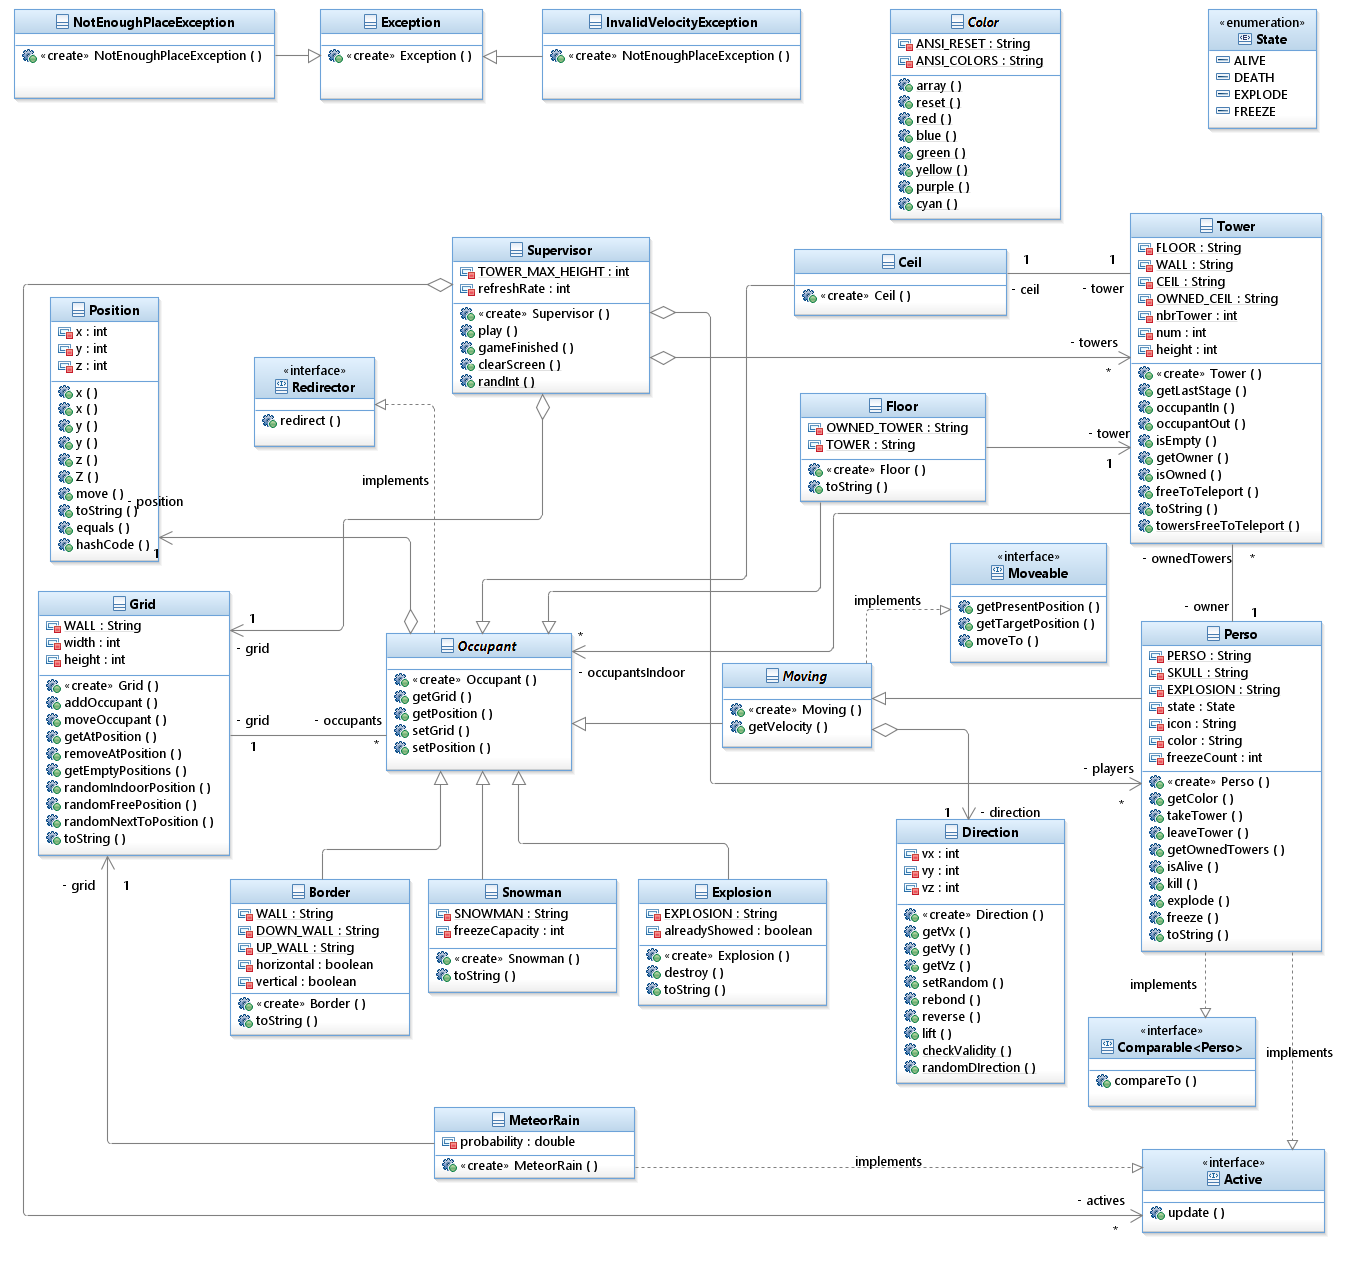
\includegraphics[width=13.9cm]{assets/pictures/ToursInfernales_Main.png}% 
  \caption{Diagramme de classes complet du projet}%
  %\label{Q1}
\end{figure}
\newpage

\section{Choix des structures de données}

Le projet \nom\~utilise plusieurs structures de données pour stocker les informations des personnages, des murs et des tours:

\begin{itemize}
    \item \emph{HashMap} $\rightarrow$ Utilisée dans la grille pour stocker les occupants tout en ayant accès à leur position en indice.
    \item \emph{List} $\rightarrow$ Utilisée notamment dans les choix aléatoires. La première structure détermine les choix possibles et la second utilise la méthode \emph{get} pour sélectionner avec un indice choisit aléatoirement. Implémentée en tant que \emph{ArrayList}.
    \item \emph{Set} $\rightarrow$ Utilisée pour renvoyer un ensemble d'objets dont le seul besoin et de parcourir la collection du début à la fin à l'aide d'un \emph{foreach}. Implémentée en tant que \emph{HashSet}.
    \item \emph{Queue} $\rightarrow$ Implémentée en tant que \emph{PriorityQueue} dans le superviseur pour déterminer l'ordre du classement des personnages.
\end{itemize}

\section{Algorithmes intéressants}

Cette section présente les algorithmes intéressants utilisés dans le projet \nom.

\subsection{Algorithme de détermination du classement final}

Dans un premier temps nous allons présenté un algorithme intéressant utilisé dans le projet \nom~. Il s'agit de l'algorithme de détermination du classement final des personnages. Cet algorithme est utilisé dans la méthode \emph{play} de la classe \emph{Supervisor} pour déterminer le classement final des personnages en fonction de leur score. 

L'algorithme utilise un tri par tas pour déterminer l'ordre du classement. On entasse puis destasse ce qui a pour effet de trier les éléments en fonction de leur priorité déterminée par la méthode \emph{compareTo}. L'algorithme est présenté dans l'encadré ci-dessous. Nous n'avons pas utiliser pour cela la méthode \emph{sort} de la classe \emph{Collections} par préférence personnel car nous n'avons pas connaissance de l'exactitude de l'algorithme utilisé dans \emph{sort}.


%%% algo 
\begin{algorithm}
\caption[\emph{Algorithme de détermination du classement final}]{\label{algo}Algorithme de détermination du classement final.}

public Perso[] play\?(int maxRound) throws InterruptedException \tab{}{
  
\dots
\bigskip


// get and return players in order using heap sort

Queue<Perso> heap = new PriorityQueue<Perso>\?();

for (Perso player: this.players) \tab{}{
  heap.add\?(player);
}

for (int i=this.players.length-1; i >= 0; i--) \tab{}{
  this.players[i] = heap.poll\?();
}

return this.players;
}
\end{algorithm}
\bigskip


\subsection{Algorithme de la pluie de météorites}

Dans un second temps nous allons présenté l'algorithme de la pluie de météorites. Cet algorithme est utilisé dans la méthode \emph{update} de la classe \emph{MeteorRain} pour déterminer si une météorite doit être lancée ou non. Il se base sur l'attribut \emph{probqbility} de la classe pour choisir avec plus ou moins de probabilité si une météorite doit être lancée ou non. Si la météorite lancée touche un personnage, elle le tue avec la méthode adaptée, sinon si la case est vide un simple spite d'explosion apparait avec une frame de durée de vie. L'algorithme est présenté dans l'encadré ci-dessous.

%%% algo 
\begin{algorithm}
  \caption[\emph{Algorithme de la pluie de météorites}]{\label{algo2}Algorithme de la pluie de météorites.}

  @Override

  public void update\?() \tab{}{
    // launch a meteor or not

    if (Math.random\?() <= this.probability) \tab{}{
      // choose a random cell and get it

      Position pos = this.grid.randomIndoorPosition\?();

      Occupant target = this.grid.getAtPosition\?(pos);

      // explode the player if it exists

      if (target instanceof Perso) \tab{}{
        Perso player = (Perso)\?target;

        if (player.isAlive\?()) \tab{}{
          player.explode\?();
        }
      }
      else if (target == null) \tab{}{
        new Explosion\?(this.grid, pos);
      }
    }
  }
\end{algorithm}%

%%%%%%%%%%%%%%%%%%%%%%%%%%%%%%%%%%%%%%%%%%%%%%%%%%%%%%%%%%%%%%%%%%%%%%%%%%%%%%%%%%%%%%%%%%%%%%%%%
%%%%%%%%%%%%%%%%%%%%%%%%%%%%%%%%%%%%%%%%   Chapitre 2   %%%%%%%%%%%%%%%%%%%%%%%%%%%%%%%%%%%%%%%%%
%%%%%%%%%%%%%%%%%%%%%%%%%%%%%%%%%%%%%%%%%%%%%%%%%%%%%%%%%%%%%%%%%%%%%%%%%%%%%%%%%%%%%%%%%%%%%%%%%
\chapter[~~~DÉVELOPPEMENT]{~~~III -~Développement de l’application}%
\label{refDev3}%

Ce chapitre explique le développement de l'application \nom\~, il détaille les points intéressants du développement, le partage du travail et ce qui a été réalisé ou non.

\section{Illustration de points intéressants}

\textcolor{cardinal}{détailler des points intéressants}


\section{Partage du travail}

\textcolor{cardinal}{partage du travail}


\section{Ce qui a été réalisé}

Cette section détaille ce qui a été réalisé dans le projet \nom\~et ce qui a été testé.

\subsection{Ce qui a été développé}

\textcolor{cardinal}{ce qui a été développé}


\subsection{Ce qui a été testé}

\textcolor{cardinal}{ce qui a été testé}


\subsection{Ce qui n'a pas été implanté}

En soit, tout ce qui a été demandé dans le sujet a été réalisé. Cependant, nous n'avons pas eu le temps (avec les autres projets et les partiels) de rendre les personnages plus intelligents, c'est-à-dire de mettre en place des stratégies sous la forme de priorité à appliquer pour les déplacements des personnages. 

Nous avons donc laissé les personnages se déplacer de manière aléatoire.%

%%%%%%%%%%%%%%%%%%%%%%%%%%%%%%%%%%%%%%%%%%%%%%%%%%%%%%%%%%%%%%%%%%%%%%%%%%%%%%%%%%%%%%%%%%%%%%%%%
%%%%%%%%%%%%%%%%%%%%%%%%%%%%%%%%%%%%%%%%   CONCLUSION   %%%%%%%%%%%%%%%%%%%%%%%%%%%%%%%%%%%%%%%%%
%%%%%%%%%%%%%%%%%%%%%%%%%%%%%%%%%%%%%%%%%%%%%%%%%%%%%%%%%%%%%%%%%%%%%%%%%%%%%%%%%%%%%%%%%%%%%%%%%
\chapter[~~~BILAN]{~~~IV -~BILAN}%
\label{cls}

Bilan technique sur les outils utilisés. Difficultés de programmation rencontrées. Présentation des améliorations possibles mais non réalisées.%

%%%%%%%%%%%%%%%%%%%%%%%%%%%%%%%%%%%%%%%%%%%%%%%%%%%%%%%%%%%%%%%%%%%%%%%%%%%%%%%%%%%%%%%%%%%%%%%%%
%%%%%%%%%%%%%%%%%%%%%%%%%%%%%%%%%%%%%%%%%   ANNEXES   %%%%%%%%%%%%%%%%%%%%%%%%%%%%%%%%%%%%%%%%%%%
%%%%%%%%%%%%%%%%%%%%%%%%%%%%%%%%%%%%%%%%%%%%%%%%%%%%%%%%%%%%%%%%%%%%%%%%%%%%%%%%%%%%%%%%%%%%%%%%%
%%% décommenter ici pour rajouter les annexes
% \input{assets/annexes}%

%%%%%%%%%%%%%%%%%%%%%%%%%%%%%%%%%%%%%%%%%%%%%%%%%%%%%%%%%%%%%%%%%%%%%%%%%%%%%%%%%%%%%%%%%%%%%%%%%
%%%%%%%%%%%%%%%%%%%%%%%%%%%%%%%%%%%%%%   BIBLIOGRAPHIE   %%%%%%%%%%%%%%%%%%%%%%%%%%%%%%%%%%%%%%%%
%%%%%%%%%%%%%%%%%%%%%%%%%%%%%%%%%%%%%%%%%%%%%%%%%%%%%%%%%%%%%%%%%%%%%%%%%%%%%%%%%%%%%%%%%%%%%%%%%
%\input{assets/bibliographie}%

%%%%%%%%%%%%%%%%%%%%%%%%%%%%%%%%%%%%%%%%%%%%%%%%%%%%%%%%%%%%%%%%%%%%%%%%%%%%%%%%%%%%%%%%%%%%%%%%%
%%%%%%%%%%%%%%%%%%%%%%%%%%%%%%%%%%%%   4eme de couverture   %%%%%%%%%%%%%%%%%%%%%%%%%%%%%%%%%%%%%
%%%%%%%%%%%%%%%%%%%%%%%%%%%%%%%%%%%%%%%%%%%%%%%%%%%%%%%%%%%%%%%%%%%%%%%%%%%%%%%%%%%%%%%%%%%%%%%%%
%\input{assets/4eme-de-couverture}%

%%%%%%%%%%%%%%%%%%%%%%%%%%%%%%%%%%%%%%%%%%%%%%%%%%%%%%%%%%%%%%%%%%%%%%%%%%%%%%%%%%%%%%%%%%%%%%%%%
%%%%%%%%%%%%%%%%%%%%%%%%%%%%%%%%%%%%%%%%%%%  END   %%%%%%%%%%%%%%%%%%%%%%%%%%%%%%%%%%%%%%%%%%%%%%
%%%%%%%%%%%%%%%%%%%%%%%%%%%%%%%%%%%%%%%%%%%%%%%%%%%%%%%%%%%%%%%%%%%%%%%%%%%%%%%%%%%%%%%%%%%%%%%%%

\bigskip % gros espace
\smallskip % patit espace
\noindent % enlève l'indentation


%%% pour faire une note en bas de page
% befib\footnote{eriughru} 

%%% pour mettre des liens 
%\url{../texmaker} %liens vers une site 
%\href{mailto:truc@bidon.org}{truc@bidon.org} %liens vers un mail


%%% pour mettre des algos
% \begin{algorithm}
%   \caption[\emph{Balise Meta pour le non-indexage d'un site}]{\label{non_indexage}Action d'affichage des voitures}
%   \Entree{Vehicule v, entier nbCases = 6 , entier tailleCanvas = 600}
%   \tcp{ \textcolor{camouflagegreen}{Fonction qui va convertir une position [i][j] en une case dans la grille}} 
%   \Act{affichageVehicules\textbf{(\textcolor{blush}{Position} pos, \textcolor{blush}{entier} tailleCanvas, \textcolor{blush}{entier} NbCases)}}{ 
%     \textcolor{blush}{entier} ct $ \leftarrow $ tailleCanvas/nbCases \\
%     \textcolor{blush}{entier} t $ \leftarrow $ tailleCanvas \\
%     afficher((pos.i*ct,pos.j*ct),(pos.i*ct+ct*t,pos.j*ct)) \\ % pour la longueur
%     afficher((pos.i*ct,pos.j*ct),(pos.i*ct,pos.j*ct+ct*t)) \\ % pour la longueur
%   }
% \end{algorithm}


%%% pour écrire dans un encadré
% \begin{center}
% \begin{boxedverbatim}
%
% \end{boxedverbatim}
% \end{center}


%%% faire une flèche
% $ \leftarrow $ 


%%% pour mettre des images (2 façons ici)
% \begin{wrapfigure}[17]{r}{0.4\columnwidth}
%   \centering%
%   \includegraphics[width=0.9\textwidth]{logoKoredge.png}% 
%    % entre crochet ce qui apparait dans la liste des figures, entre acolade ce qui pparait en dessous de la figure
%   \caption[\emph{Titre}]{ \emph{Titre} légende, (source)}
%   \label{Tux}%
% \end{wrapfigure}

% \newpage
% Rush-Hour est un jeu de type casse-tête créé par Nob Yoshigahara à la fin des années 1970. Initialement un jeu de plateau, son succès a permis l'adaptation du jeu de société en jeu vidéo. Le but du jeu est simple: réussir à faire sortir la voiture principale de la grille en déplaçant les véhicules qui bloquent la voiture, le tout en un minimum de mouvements. A partir de ce nombre de mouvements, le joueur peut décrocher entre trois à une étoile selon son score.
% Dans le tableau~\ref{Tux}, page~\pageref{Tux}, nous lisons
% \begin{figure}[!ht]
%   \centering% 
%   \includegraphics[width=0.6\textwidth]{logoKoredge.png}
%   \caption{Titre légende, (source) }%
%   \label{Tux2}
% \end{figure}
% Rush-Hour est un jeu de type casse-tête créé par Nob Yoshigahara à la fin des années 1970. Initialement un jeu de plateau, son succès a permis l'adaptation du jeu de société en jeu vidéo. Le but du jeu est simple: réussir à faire sortir la voiture principale de la grille en déplaçant les véhicules qui bloquent la voiture, le tout en un minimum de mouvements. A partir de ce nombre de mouvements, le joueur peut décrocher entre trois à une étoile selon son score.
% Dans le tableau~\ref{Tux2}, page~\pageref{Tux2}, nous lisons


%%% toutes les couleurs:
% \textcolor{camouflagegreen}{\textsc{camouflagegreen}}
% \textcolor{babyblueeyes}{\textsc{babyblueeyes}}
% \textcolor{blush}{\textsc{blush}}
% \textcolor{chromeyellow}{\textsc{chromeyellow}}
% \textcolor{cardinal}{\textsc{cardinal}}
% \textcolor{purple}{\textsc{purple}}
% \color{blue}{blue}
% \color{brown}{brown}
% \color{cyan}cyan
% \color{darkgray}darkgray
% \color{gray}gray
% \color{green}green
% \color{lightgray}lightgray
% \color{lime}lime
% \color{magenta}magenta
% \color{olive}olive
% \color{orange}orange
% \color{pink}pink
% \color{purple}purple
% \color{red}red
% \color{teal}teal
% \color{violet}violet
% \color{yellow}yellow
% \color{black}black
% \newpage
\end{document}